\documentclass[13pt]{beamer}

\theoremstyle{plain}% default
\newtheorem{teo}{Teorema}[section]
\newtheorem{lem}[teo]{Lema}
\newtheorem{prop}{Proposição}
\newtheorem{cor}[teo]{Corolário}

\theoremstyle{definition}
\newtheorem{defn}{Definição}[section]
\newtheorem{conj}{Conjectura}[section]
\newtheorem{exmp}{Exemplo}

\theoremstyle{remark}
\newtheorem*{rem}{Observação}
\newtheorem*{note}{Nota}
\newtheorem{case}{Caso}


% Macros

\renewcommand{\vec}[1]{\mathbf{#1}}
\newcommand{\K}{\mathbb{K}}
\newcommand{\I}{\mathbb{I}}
\DeclarePairedDelimiter{\dotprod}{\langle}{\rangle}
\DeclareMathOperator{\rk}{rk}
\DeclareMathOperator{\intt}{int}
\DeclareMathOperator{\diam}{diam}
\DeclareMathOperator{\rref}{rref}
\DeclareMathOperator{\vspan}{span}
\DeclareMathOperator{\proj}{proj}
\usepackage{global-macros}

\begin{comment}
    Estrutura:
     - Slide inicial
        -- Falar por alto a ideia do Teorema.
     - Explicar o que é uma rede neural
        -- Blá blá sobre inspiração nos neurônios do cérebro
        -- Imagem clássica da feedforward network
        % -- Link para os vídeos do 3b1b
     - Apliações de redes neurais
        -- Citar algumas aplicações bem sucedidas (links para wikipédia)
        -- Reforçar a importância do TAU
     - Mostrar artigo do Cybenko
        -- Enunciar Teorema igual na introdução do relatório
        -- Referência do Artigo
        -- Print da demonstração
     - Interludio: começar mais de baixo
        -- Apresentar Weirstrass e Hilbert
        -- Explicar por que estudar esses resultados antes
            --- TAU muito avançado para o que eu sabia
            --- Curso de medida ainda começando
            --- Interessante estudar aproximadores em contextos
                mais simples
     - Aproximação de Weierstrass
       -- Contexto mais simples
       -- Enunciar Teorema
       -- Já introduzir norma infinito e notação
       -- Dar ideia da demonstração, usando polinômios de bernstein
     - Ilustrar Weierstrass
       -- Mostrar polinômios de Bernstein aproximando uma função ****
     - Hilbert
       -- Introduzir problema, falar brevemente sobre como ele foi
          formulado inicialmente
       -- Falar um pouco da história do resultado
       -- Comentar sobre diferenças com relação aos teoremas anteriores
           --- Aproximação vs Representação Exata
     - Tentar dar uma ideia da demonstração do 13 de Hilbert
     - Fim do interlúdio: Volta ao TAU
       -- Fazer diagrama ilustrando resultados necessários para mostrar o TAU
     % - Pincelada da Prova
     %   -- Fornecer principais passos da demonstração em tópicos, mostrando onde
     %      cada Teorema é Utilizado
     %   -- Falar sobre lema que contém boa parte da demonstração (sigmoide é
     %      discriminatória)
     - Hahn Banach
       -- Enunciar Teorema, falar um pouco da importância dele
       -- Falar sobre resultados necessários para prová-lo
       -- Ilustrar de alguma forma o Teorema
     - Enunciar o corolário que realmente vai ser utilizado na prova do TAU
       -- Dar ideia da demonstração
     - Representação de Riesz
       -- Falar sobre diferentes versões do Teorema
       --- Em Análise Funcional (Espaços de Hilbert)
           --- Em Teorema da Medida (Espaços L_p)
           --- No contexto do TAU
       -- Enunciar Teorema que o Cybenko usa, falar que tava fora da minha alçada
       -- Enunciar versão mais simples, dar ideia da demonstração
     - Reapresentar demonstração do TAU
       -- Falar do Lema
     - Enunciar lema e dar ideia da demonstração
     - Ilustrar TAU com um exemplo mais de boa, por exemplo alguma função real
       em R² ****
     - Problemas do TAU
       -- Falar de bounds para o número de neurônios na camada intermediária
       -- Problema de achar a rede que aproxima a função (SGD)
     - Generalizações
        -- Comentar sobre resultados relativos a aproximação de derivadas
     - Falar de próximos passos da IC
       -- DGM
     - Link para Repositório do Github
     - Agradecimentos
       -- Yuri, CNPq
\end{comment}

\title[Teorema da Aproximação Universal]{Sobre o Teorema da Aproximação Universal}
% \author[C. Lins]{{Caio Lins }}
\author[C. Lins]{Caio Lins \texorpdfstring{\\}{}[1ex]  {\small Orientador: Yuri Saporito}}
%%     {\and} 
%%     {\textit{Orientador}} 
%%     {Yuri Saporito}}
\institute[EMAp]{FGV - EMAp}
\date[EMAp 2021]{Outubro 2021}
\logo{
\includegraphics[height=0.8cm]{../figuras/fgv_logo.png}}


\begin{document}

\maketitle

%%%%%%%%%%%%%%%%%%%%%%%%%%%%%%%%%%%%%%%%%%%%%%%%%%%%%%%%%%%
%%%%%%%%%%%%%%% Intro a Redes Neurais %%%%%%%%%%%%%%%%%%%%%
%%%%%%%%%%%%%%%%%%%%%%%%%%%%%%%%%%%%%%%%%%%%%%%%%%%%%%%%%%%

\begin{frame}{Overview de Redes Neurais}{O que são redes neurais?}
    \begin{itemize}
        \item Redes neurais são funções inspiradas em um modelo do funcionamento do cérebro humano.
            São organizadas em camadas de ``neurônios''.
    \end{itemize}
    \begin{figure}
        \begin{center}
            % !TeX root = ../main.tex

\tikzset{%
  every neuron/.style={
    circle,
    draw,
    minimum size=1cm
  },
  neuron missing/.style={
    draw=none, 
    scale=3,
    text height=0.3cm,
    execute at begin node=\color{black}$\vdots$
  },
}

\vspace{.6cm}

\begin{tikzpicture}[x=1.5cm, y=1.5cm, yshift=-1, >=stealth]

\foreach \m/\l [count=\y] in {1,missing,2}
  \node [every neuron/.try, neuron \m/.try] (input-\m) at (0,1.75-\y) {};

\foreach \m [count=\y] in {1,missing,2}
  \node [every neuron/.try, neuron \m/.try ] (hidden-\m) at (2,2.25-\y*1.25) {};

\foreach \m [count=\y] in {1}
  \node [every neuron/.try, neuron \m/.try ] (output-\m) at (4,1-\y) {};

\foreach \l [count=\i] in {1,n}
  \draw [<-] (input-\i) -- ++(-1,0)
    node [above, midway] {$x_\l$};

%% \foreach \l [count=\i] in {1,n}
%%   \node [above] at (hidden-\i.north) {$H_\l$};
\node [above] at (hidden-1.north) {\( \sigma (y_{ 1 }^{ T }x + \theta_{ 1 }) \)};
\node [below] at (hidden-2.south) {\( \sigma (y_{ N }^{ T }x + \theta_{ N }) \)};

\foreach \l [count=\i] in {1}
  \draw [->] (output-\i) -- ++(3,0)
    node [above, midway] {\( \sum_{ j=1 }^{ N } \alpha_{ j } \sigma (y_{ j }^{ T } + \theta_{ j }) \)};

%% \foreach \i in {1,...,2}
%%   \foreach \j in {1,...,2}
%%     \draw [->] (input-\i) -- (hidden-\j)
%%         node [above,pos=.2] {\( y_{ 1 }^{ (1) } \)};
\draw [->] (input-1) -- (hidden-1)
    node [above, pos=.3] {\( w_{ 1,1 } \)};
\draw [->] (input-2) -- (hidden-1)
    node [above, pos=.2, xshift=-2mm] {\( w_{ n,1 } \)};
\draw [->] (input-1) -- (hidden-2)
    node [above, pos=.2,xshift=2mm] {\( w_{ 1,N } \)};
\draw [->] (input-2) -- (hidden-2)
    node [above, pos=.3] {\( w_{ n,N } \)};

%% \foreach \i in {1,...,2}
%%   \foreach \j in {1}
%%     \draw [->] (hidden-\i) -- (output-\j);
\draw [->] (hidden-1) -- (output-1)
    node [above, midway] {\( \alpha_{ 1 } \)};
\draw [->] (hidden-2) -- (output-1)
    node [below, midway, yshift=-1mm] {\( \alpha_{ N } \)};

\foreach \l [count=\x from 0] in {de Input, Intermediária, de Ouput}
  \node [align=center, above] at (\x*2,2) {Camada \\ \l};

\end{tikzpicture}
        \end{center}
    \end{figure}
\end{frame}

\begin{frame}{Overview de Redes Neurais}{O que são redes neurais?}
    \begin{itemize}
        \item Input: \( \bfx = ( x_{ 1 }, \dots, x_{ n } ) \in \R^{ n } \).
        \item Pesos (\emph{weights}): \( \bfw_{ j } = ( w_{ 1, j }, \dots, w_{ n, j } ) \in \R^{ n }, j = 1, \dots, N \).
        \item Viéses (\emph{biases}): \( \theta_{ j } \in \R , j = 1, \dots, N\).
        \item Função de ativação: \( \sigma : \R \to \R \).
    \end{itemize}
    \begin{center}
        % !TeX root = ../main.tex

\tikzset{%
  every neuron/.style={
    circle,
    draw,
    minimum size=1cm
  },
  neuron missing/.style={
    draw=none, 
    scale=3,
    text height=0.3cm,
    execute at begin node=\color{black}$\vdots$
  },
}

\vspace{.6cm}

\begin{tikzpicture}[x=1.5cm, y=1.5cm, yshift=-1, >=stealth]

\foreach \m/\l [count=\y] in {1,missing,2}
  \node [every neuron/.try, neuron \m/.try] (input-\m) at (0,1.75-\y) {};

\foreach \m [count=\y] in {1,missing,2}
  \node [every neuron/.try, neuron \m/.try ] (hidden-\m) at (2,2.25-\y*1.25) {};

\foreach \m [count=\y] in {1}
  \node [every neuron/.try, neuron \m/.try ] (output-\m) at (4,1-\y) {};

\foreach \l [count=\i] in {1,n}
  \draw [<-] (input-\i) -- ++(-1,0)
    node [above, midway] {$x_\l$};

%% \foreach \l [count=\i] in {1,n}
%%   \node [above] at (hidden-\i.north) {$H_\l$};
\node [above] at (hidden-1.north) {\( \sigma (y_{ 1 }^{ T }x + \theta_{ 1 }) \)};
\node [below] at (hidden-2.south) {\( \sigma (y_{ N }^{ T }x + \theta_{ N }) \)};

\foreach \l [count=\i] in {1}
  \draw [->] (output-\i) -- ++(3,0)
    node [above, midway] {\( \sum_{ j=1 }^{ N } \alpha_{ j } \sigma (y_{ j }^{ T } + \theta_{ j }) \)};

%% \foreach \i in {1,...,2}
%%   \foreach \j in {1,...,2}
%%     \draw [->] (input-\i) -- (hidden-\j)
%%         node [above,pos=.2] {\( y_{ 1 }^{ (1) } \)};
\draw [->] (input-1) -- (hidden-1)
    node [above, pos=.3] {\( w_{ 1,1 } \)};
\draw [->] (input-2) -- (hidden-1)
    node [above, pos=.2, xshift=-2mm] {\( w_{ n,1 } \)};
\draw [->] (input-1) -- (hidden-2)
    node [above, pos=.2,xshift=2mm] {\( w_{ 1,N } \)};
\draw [->] (input-2) -- (hidden-2)
    node [above, pos=.3] {\( w_{ n,N } \)};

%% \foreach \i in {1,...,2}
%%   \foreach \j in {1}
%%     \draw [->] (hidden-\i) -- (output-\j);
\draw [->] (hidden-1) -- (output-1)
    node [above, midway] {\( \alpha_{ 1 } \)};
\draw [->] (hidden-2) -- (output-1)
    node [below, midway, yshift=-1mm] {\( \alpha_{ N } \)};

\foreach \l [count=\x from 0] in {de Input, Intermediária, de Ouput}
  \node [align=center, above] at (\x*2,2) {Camada \\ \l};

\end{tikzpicture}
    \end{center}
\end{frame}

\begin{frame}{Overview de Redes Neurais}{O que são redes neurais?}
    \vspace{2pt}
    O \( j \)-ésimo neurônio da camada oculta computa a soma
    \begin{equation*}
        \bfw_{ j }^{ \transpose } \bfx + \theta_{ j } = w_{ 1, j }x_{ 1 } + w_{ 2,j } x_{ 2 } + \cdots + w_{ n, j } x_{ n } + \theta_{ j }
    \end{equation*}
    e passa o resultado pela ativação \( \sigma : \R \to \R \), que é \emph{não linear}.
    \begin{center}
        % !TeX root = ../main.tex

\tikzset{%
  every neuron/.style={
    circle,
    draw,
    minimum size=1cm
  },
  neuron missing/.style={
    draw=none, 
    scale=3,
    text height=0.3cm,
    execute at begin node=\color{black}$\vdots$
  },
}

\vspace{.6cm}

\begin{tikzpicture}[x=1.5cm, y=1.5cm, yshift=-1, >=stealth]

\foreach \m/\l [count=\y] in {1,missing,2}
  \node [every neuron/.try, neuron \m/.try] (input-\m) at (0,1.75-\y) {};

\foreach \m [count=\y] in {1,missing,2}
  \node [every neuron/.try, neuron \m/.try ] (hidden-\m) at (2,2.25-\y*1.25) {};

\foreach \m [count=\y] in {1}
  \node [every neuron/.try, neuron \m/.try ] (output-\m) at (4,1-\y) {};

\foreach \l [count=\i] in {1,n}
  \draw [<-] (input-\i) -- ++(-1,0)
    node [above, midway] {$x_\l$};

%% \foreach \l [count=\i] in {1,n}
%%   \node [above] at (hidden-\i.north) {$H_\l$};
\node [above] at (hidden-1.north) {\( \sigma (y_{ 1 }^{ T }x + \theta_{ 1 }) \)};
\node [below] at (hidden-2.south) {\( \sigma (y_{ N }^{ T }x + \theta_{ N }) \)};

\foreach \l [count=\i] in {1}
  \draw [->] (output-\i) -- ++(3,0)
    node [above, midway] {\( \sum_{ j=1 }^{ N } \alpha_{ j } \sigma (y_{ j }^{ T } + \theta_{ j }) \)};

%% \foreach \i in {1,...,2}
%%   \foreach \j in {1,...,2}
%%     \draw [->] (input-\i) -- (hidden-\j)
%%         node [above,pos=.2] {\( y_{ 1 }^{ (1) } \)};
\draw [->] (input-1) -- (hidden-1)
    node [above, pos=.3] {\( w_{ 1,1 } \)};
\draw [->] (input-2) -- (hidden-1)
    node [above, pos=.2, xshift=-2mm] {\( w_{ n,1 } \)};
\draw [->] (input-1) -- (hidden-2)
    node [above, pos=.2,xshift=2mm] {\( w_{ 1,N } \)};
\draw [->] (input-2) -- (hidden-2)
    node [above, pos=.3] {\( w_{ n,N } \)};

%% \foreach \i in {1,...,2}
%%   \foreach \j in {1}
%%     \draw [->] (hidden-\i) -- (output-\j);
\draw [->] (hidden-1) -- (output-1)
    node [above, midway] {\( \alpha_{ 1 } \)};
\draw [->] (hidden-2) -- (output-1)
    node [below, midway, yshift=-1mm] {\( \alpha_{ N } \)};

\foreach \l [count=\x from 0] in {de Input, Intermediária, de Ouput}
  \node [align=center, above] at (\x*2,2) {Camada \\ \l};

\end{tikzpicture}
    \end{center}
\end{frame}

\begin{frame}{Overview de Redes Neurais}{O que são redes neurais?}
    \vspace{2pt}
    Existem várias funções de ativação possíveis, mas tenham em mente a \emph{função logística}:
    \begin{equation*}
        \sigma ( x ) = \frac{ 1 }{ 1 + e^{ -x } }
    .\end{equation*}
    \begin{center}
        \begin{tikzpicture}[scale=1]
    \begin{axis}[
        axis x line=middle,
        axis y line=middle,
        yscale=.6,
        ylabel=\( \sigma ( x ) \),
        ytick={1},
        yticklabels={1},
        y label style={anchor=west},
        xlabel=\( x \),
        samples=200
    ]
    \addplot[domain=-10:10, blue, thick] {1/(1 + e^(-x))};
    \end{axis}
\end{tikzpicture}

    \end{center}
\end{frame}

\begin{frame}{Overview de Redes Neurais}{O que são redes neurais?}
    \vspace{2pt}
    Neste caso, o output da rede é um escalar, dado pela soma:
    \(
        G ( \bfx ) = \sum_{ j=1 }^{ N } \alpha_{ j } \sigma ( \bfw_{ j }^{ \transpose } \bfx + \theta_{ j } )
        \),
    mas isso não é regra.
    \begin{center}
        % !TeX root = ../main.tex

\tikzset{%
  every neuron/.style={
    circle,
    draw,
    minimum size=1cm
  },
  neuron missing/.style={
    draw=none, 
    scale=3,
    text height=0.3cm,
    execute at begin node=\color{black}$\vdots$
  },
}

\vspace{.6cm}

\begin{tikzpicture}[x=1.5cm, y=1.5cm, yshift=-1, >=stealth]

\foreach \m/\l [count=\y] in {1,missing,2}
  \node [every neuron/.try, neuron \m/.try] (input-\m) at (0,1.75-\y) {};

\foreach \m [count=\y] in {1,missing,2}
  \node [every neuron/.try, neuron \m/.try ] (hidden-\m) at (2,2.25-\y*1.25) {};

\foreach \m [count=\y] in {1}
  \node [every neuron/.try, neuron \m/.try ] (output-\m) at (4,1-\y) {};

\foreach \l [count=\i] in {1,n}
  \draw [<-] (input-\i) -- ++(-1,0)
    node [above, midway] {$x_\l$};

%% \foreach \l [count=\i] in {1,n}
%%   \node [above] at (hidden-\i.north) {$H_\l$};
\node [above] at (hidden-1.north) {\( \sigma (y_{ 1 }^{ T }x + \theta_{ 1 }) \)};
\node [below] at (hidden-2.south) {\( \sigma (y_{ N }^{ T }x + \theta_{ N }) \)};

\foreach \l [count=\i] in {1}
  \draw [->] (output-\i) -- ++(3,0)
    node [above, midway] {\( \sum_{ j=1 }^{ N } \alpha_{ j } \sigma (y_{ j }^{ T } + \theta_{ j }) \)};

%% \foreach \i in {1,...,2}
%%   \foreach \j in {1,...,2}
%%     \draw [->] (input-\i) -- (hidden-\j)
%%         node [above,pos=.2] {\( y_{ 1 }^{ (1) } \)};
\draw [->] (input-1) -- (hidden-1)
    node [above, pos=.3] {\( w_{ 1,1 } \)};
\draw [->] (input-2) -- (hidden-1)
    node [above, pos=.2, xshift=-2mm] {\( w_{ n,1 } \)};
\draw [->] (input-1) -- (hidden-2)
    node [above, pos=.2,xshift=2mm] {\( w_{ 1,N } \)};
\draw [->] (input-2) -- (hidden-2)
    node [above, pos=.3] {\( w_{ n,N } \)};

%% \foreach \i in {1,...,2}
%%   \foreach \j in {1}
%%     \draw [->] (hidden-\i) -- (output-\j);
\draw [->] (hidden-1) -- (output-1)
    node [above, midway] {\( \alpha_{ 1 } \)};
\draw [->] (hidden-2) -- (output-1)
    node [below, midway, yshift=-1mm] {\( \alpha_{ N } \)};

\foreach \l [count=\x from 0] in {de Input, Intermediária, de Ouput}
  \node [align=center, above] at (\x*2,2) {Camada \\ \l};

\end{tikzpicture}
    \end{center}
\end{frame}

\begin{frame}{Overview de Redes Neurais}{O que são redes neurais?}
    \vspace{2pt}
    A rede mostrada até o momento tem apenas uma camada oculta, mas redes neurais em geral têm várias.
    \begin{center}
        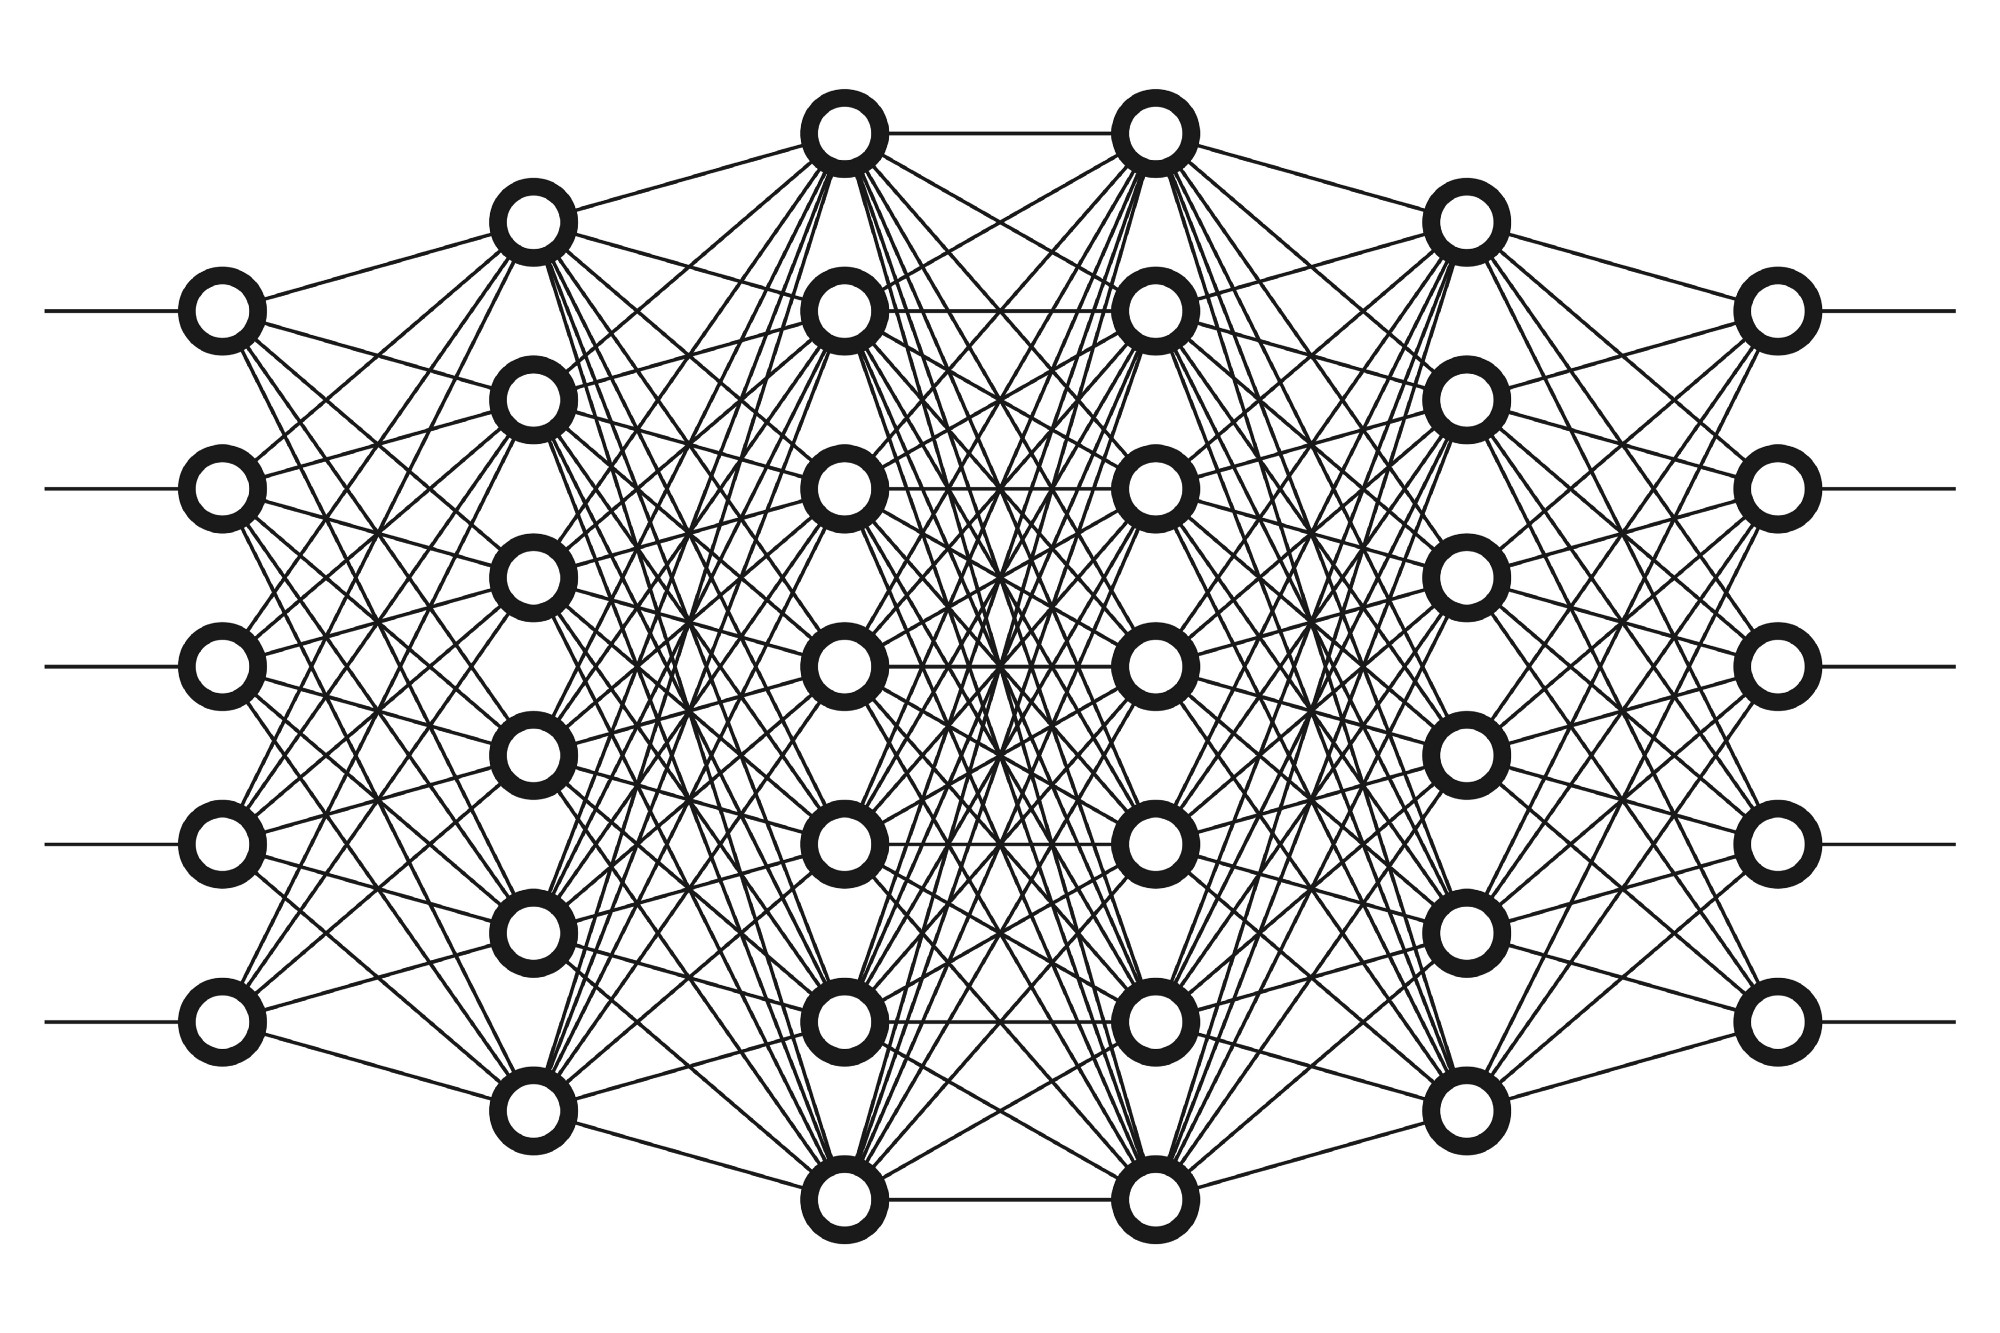
\includegraphics[width=.7\textwidth]{../figuras/multi-layer-neural-network.jpeg}
    \end{center}
\end{frame}

\begin{frame}{Overview de Redes Neurais}{Para que servem?}
    \vspace{2pt}
    Diversas aplicações:
    \begin{itemize}
        \item Classificação de imagens, incluindo reconhecimento facial;
        \item Predição de séries temporais;
        \item Análise de regressão;
        \item O algoritmo usado pela inteligência artificial \emph{AlphaGo} emprega redes neurais convolucionais (CNNs).
        \item Deep Galerkin Method (DGM): Algoritmo de Deep Learning para resolver equações diferenciais parciais.
    \end{itemize}
\end{frame}

%%%%%%%%%%%%%%%%%%%%%%%%%%%%%%%%%%%%%%%%%%%%%%%%%%%%%%%%%%%
%%%%%%% The vital question: Faz sentido tudo isso? %%%%%%%%
%%%%%%%%%%%%%%%%%%%%%%%%%%%%%%%%%%%%%%%%%%%%%%%%%%%%%%%%%%%

\begin{frame}{Redes Neurais Funcionam?}
    \begin{itemize}
        \item<1-> Podemos nos questionar se Redes Neurais são capazes de realizar essas tarefas arbitrariamente bem (no fundo, tudo se resume a aproximar funções).
        \item<2-> A resposta é sim.
    \end{itemize}
\end{frame}

\begin{frame}{Redes Neurais Funcionam?}
    \begin{TAU}
        Seja \( \sigma : \R \to \R \) uma função contínua e discriminatória qualquer.
        Então, dada uma função \( f : [0, 1]^{ n } \to \R \) contínua, e um \( \varepsilon > 0 \), existe uma função \( G : [0, 1]^{ n } \to \R \), da seguinte forma:
        \begin{equation*}
            G ( \bfx ) = \sum_{ j=1 }^{ N } \alpha_{ j } \sigma ( \bfw_{ j }^{ \transpose } \bfx + \theta_{ j } )
        ,\end{equation*}
        onde \( \alpha_{ j }, \theta_{ j } \in \R \) e \( \bfw_{ j } \in \R^{ n } \), \( j = 1, \dots, N \), tal que
        \begin{equation*}
            \abs{ G ( \bfx ) - f ( \bfx ) } < \varepsilon
        \end{equation*}
        para todo \( \bfx \in [0, 1]^{ n } \).
    \end{TAU}
\end{frame}

\begin{frame}{Redes Neurais Funcionam?}
    \begin{itemize}
        \item<1-> Mais à frente especificaremos o que significa ``discriminatória''.
        \item<2-> Ou seja, redes neurais com uma camada oculta são aproximadores universais de funções reais contínuas definidas em \( [0, 1]^{ n } = \vcentcolon \I^{ n } \).
    \end{itemize}
\end{frame}

\begin{frame}{Redes Neurais Funcionam?}
    \begin{itemize}
        \item<1-> Artigo onde esse resultado foi provado: ``Approximation by superpositions of a sigmoidal function'' \cite{cybenko89}
    \end{itemize}
    \begin{center}
        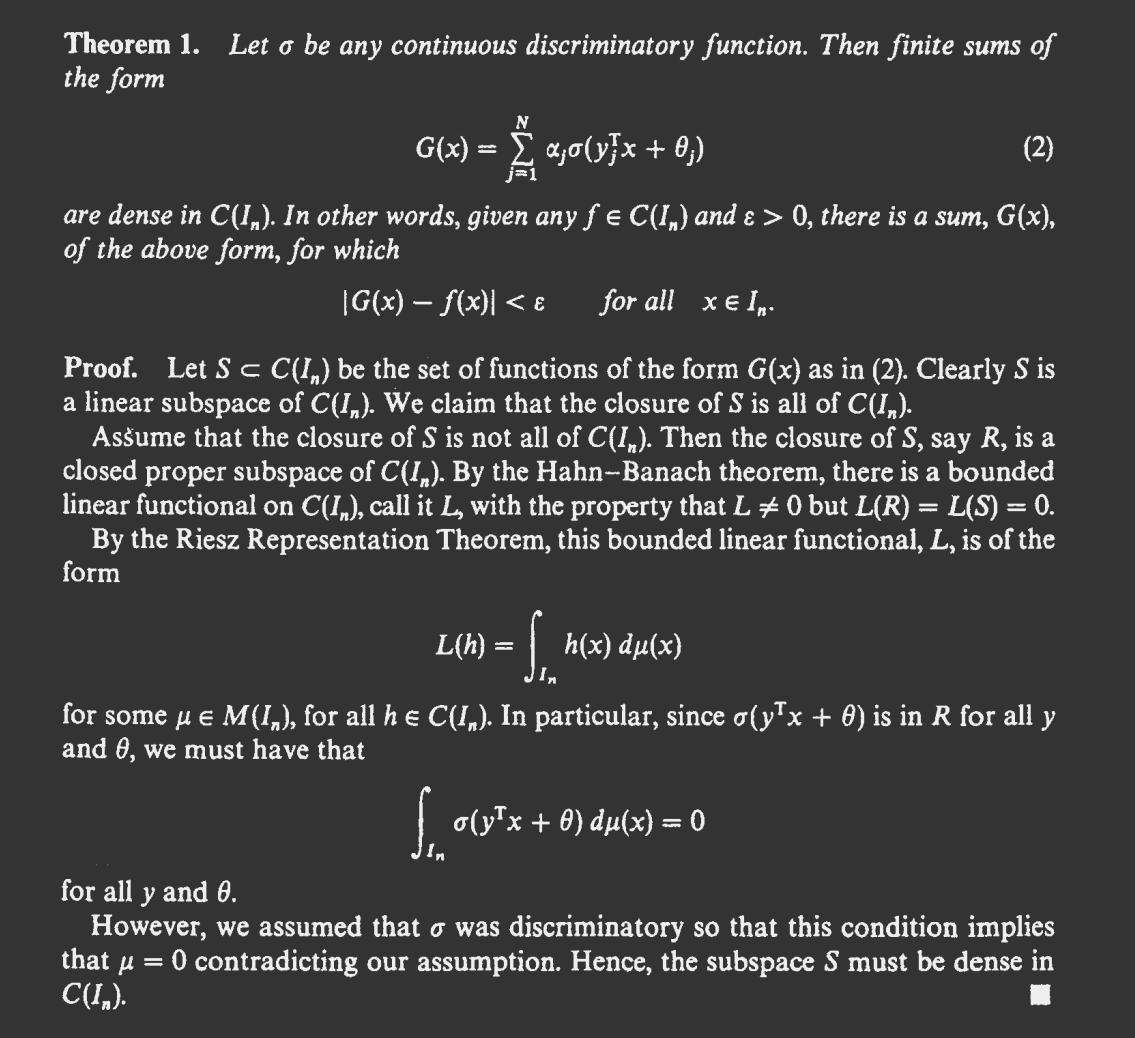
\includegraphics[width=.7\textwidth]{../figuras/cybenko.png}
    \end{center}
\end{frame}

%%%%%%%%%%%%%%%%%%%%%%%%%%%%%%%%%%%%%%%%%%%%%%%%%%%%%%%%%%%
%%%%%%%%%%%% Interlúdio: Weierstrass e Hilbert %%%%%%%%%%%%
%%%%%%%%%%%%%%%%%%%%%%%%%%%%%%%%%%%%%%%%%%%%%%%%%%%%%%%%%%%

\begin{frame}{Interlúdio}{Outros resultados relacionados}
    \begin{itemize}
        \item<1-> Demonstração utiliza resultados de Análise Funcional e Teoria da Medida.
        \item<2-> Estudar aproximações em outros contextos
            \begin{itemize}
                \item<3-> Teorema da Aproximação de Weierstrass:
                    \begin{itemize}
                        \item<4-> \emph{Aproximar} funções contínuas de um intervalo na reta por meio de \emph{polinômios}.
                    \end{itemize}
                \item<5-> Um desdobramento do \( 13^{ \circ } \) problema de Hilbert:
                    \begin{itemize}
                        \item<6-> Representar \emph{de maneira exata} funções contínuas de \( \I^{ n } \) em \( \R \) por meio de composições e adições de \emph{funções contínuas de \( \R \) em \( \R \)}.
                    \end{itemize}
            \end{itemize}
    \end{itemize}
\end{frame}

\begin{frame}{Interlúdio}{Teorema da Aproximação de Weierstrass}
    Um pouco de notação:
    \begin{itemize}
        \item Dado \( X \subseteq \R^{ n } \), definimos
            \begin{equation*}
                C ( X ) = \left\{ \varphi : X \to \R \mid \varphi \text{ é contínua } \right\}
            .\end{equation*}
        \item \( C ( X ) \) é um espaço vetorial no qual introduzimos a seguinte norma:
            \begin{equation*}
                \norm{ \varphi }_{ \infty } \defeq \sup \left\{ \abs{ \varphi ( x ) } : x \in X \right\}
            .\end{equation*}
    \end{itemize}
\end{frame}

\begin{frame}{Interlúdio}{Teorema da Aproximação de Weierstrass}
    \begin{teo*}[Aproximação de Weierstrass]
        Dada \( f \in C ( [a, b] ) \), para todo \( \varepsilon > 0 \) existe um polinômio \( p : [a, b] \to \R \) tal que
        \begin{equation*}
            \norm{ f - p }_{ \infty } < \varepsilon
        .\end{equation*}
    \end{teo*}
\end{frame}

\begin{frame}{Interlúdio}{Teorema da Aproximação de Weierstrass}
    Ideia da demonstração \cite{weierstrass}:
    \begin{itemize}
        \item<1-> Reduzir ao caso em que \( [a, b] = [0, 1] \).
        \item<2-> Aproximar \( f \) pelos seus \emph{Polinômios de Bernstein}:
            \begin{equation*}
                B_{ n } ( x, f ) \defeq \sum_{ k=0 }^{ n } f
                \left( \frac{ k }{ n } \right)
                \binom{n}{k}
                x^{ k }
                ( 1 - x )^{ n - k }
            .\end{equation*}
        \item<3-> De fato, temos
            \begin{equation*}
                \lim_{ n \to \infty } \norm{ B_{ n } ( \cdot, f ) - f }_{ \infty } = 0
            .\end{equation*}
    \end{itemize}
\end{frame}

\begin{frame}{Interlúdio}{Teorema da Aproximação de Weierstrass}
    \vspace{3pt}
    Ilustrando o Teorema:
    \begin{center}
        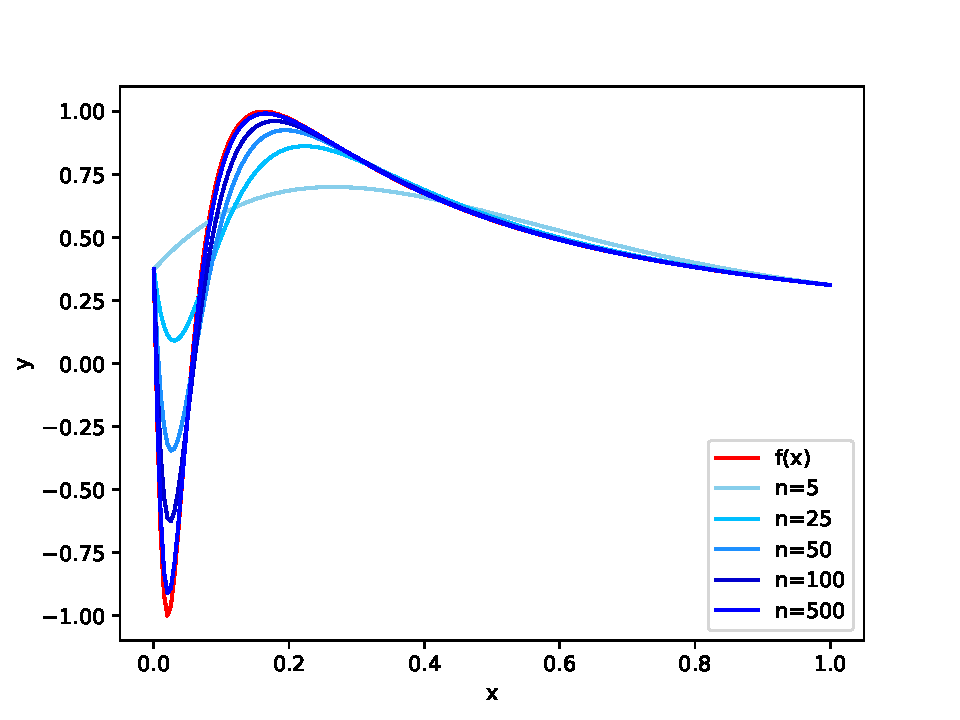
\includegraphics[width=.75\textwidth]{../figuras/weierstrass_seno.pdf}
        \( f ( x ) = \sen \left( \frac{ 1 }{ 3 ( x + 0.05 ) } \right) \)
    \end{center}
\end{frame}

\begin{frame}{Interlúdio}{Teorema da Aproximação de Weierstrass}
    \vspace{3pt}
    Ilustrando o Teorema:
    \begin{center}
        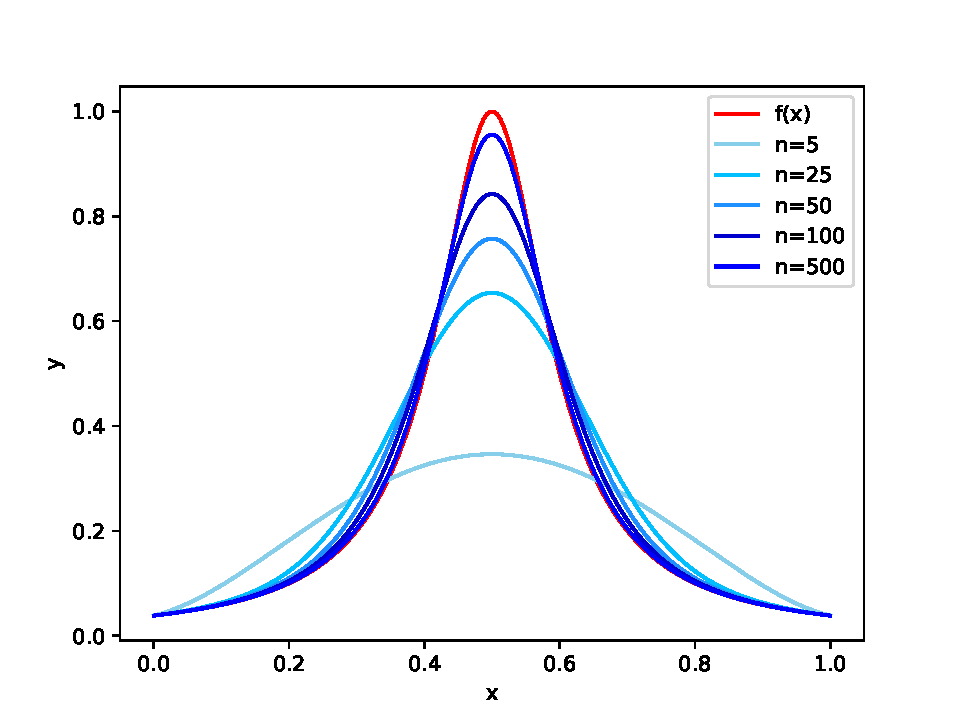
\includegraphics[width=.75\textwidth]{../figuras/weierstrass_cauchy.pdf}
        \( f ( x ) = \frac{ 1 }{ 100 ( x - 0.5 )^2 + 1 } \)
    \end{center}
\end{frame}

\begin{frame}{Interlúdio}{Teorema da Aproximação de Weierstrass}
    \vspace{3pt}
    Um exemplo com \( f \) descontínua:
    \begin{center}
        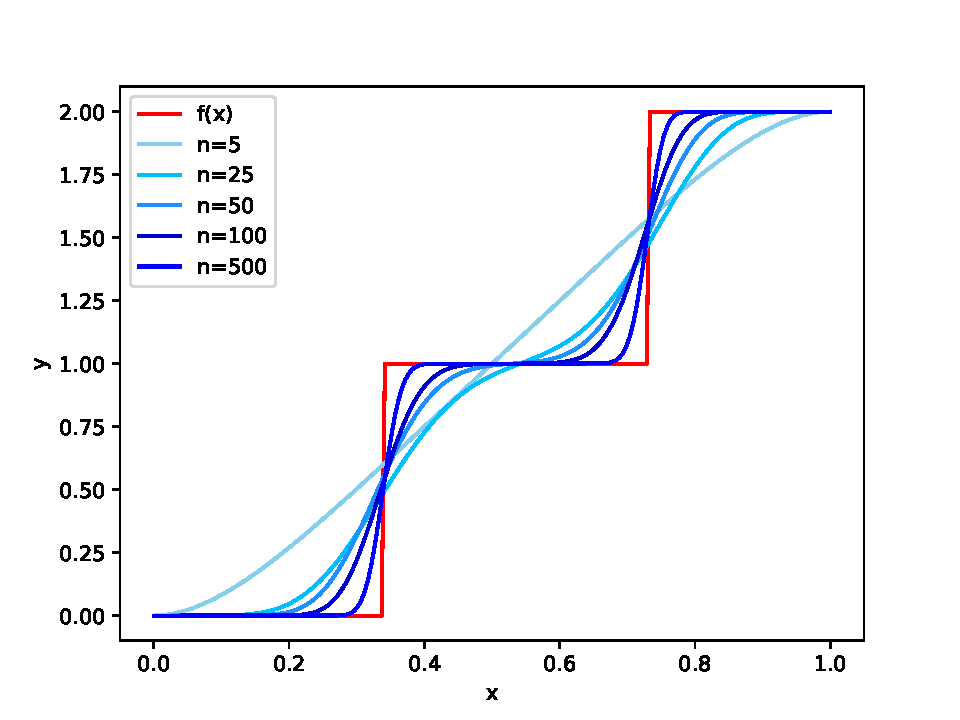
\includegraphics[width=.75\textwidth]{../figuras/weierstrass_cobrinha.pdf}
        \( f ( x ) = \abs{ \floor{3\sen ( x )} } \)
    \end{center}
\end{frame}

\begin{frame}{Interlúdio}{\( 13^{ \circ } \) problema de Hilbert}
    \begin{itemize}
        \item Com a linguagem da época, Hilbert conjecturou que existem funções contínuas \( f : \I^{ 3 } \to \R \) que não podem ser representadas como composições e somas de funções contínuas de \( \R \to \R \) \cite{hilbert}.
        \item<2-> Exemplo em \( \I^{ 2 } \): \( f ( x, y ) = xy \).
            Observe que
            \begin{align*}
                \visible<3->{f ( x, y) &= xy = ( x+1 ) ( y+1 ) - \left(x + \frac{ 1 }{ 2 }\right) - \left(y + \frac{ 1 }{ 2 }\right) \\}
                \visible<4->{&= e^{ [ \log ( x + 1 ) + \log ( y+1 ) ] } - \left(x + \frac{ 1 }{ 2 }\right) - \left(y + \frac{ 1 }{ 2 }\right)}
            .\end{align*}
            \visible<5->{(Somamos \( 1 \) para evitar \( \log 0 \)).}
    \end{itemize}
\end{frame}

\begin{frame}{Interlúdio}{\( 13^{ \circ } \) problema de Hilbert}
    \begin{itemize}
        \item<1-> Essa conjectura era \textbf{falsa}.
            \begin{itemize}
                \item<2-> Provado por Vladimir Igorevich Arnol'd em 1957, baseado no trabalho de seu orientador, Andrej Nikolajewitseh Kolmogorov.
            \end{itemize}
        \item<3-> Teorema da Superposição de Kolmogorov.
        \item<4-> Foi generalizado posteriormente.
    \end{itemize}
\end{frame}

\begin{frame}{Interlúdio}{\( 13^{ \circ } \) problema de Hilbert}
    \begin{teo*}[Kolmogorov, Arnol'd, Kahane, Lorentz e Sprechner]
        Para todo \( n \in \N \) com \( n \geq 2 \), existem números reais \( \lambda_{ 1 }, \lambda_{ 2 }, \dots, \lambda_{ n } \) e funções contínuas \( \varphi_{ k } : \I \to \R \), para \( k = 1, \dots, 2n+1 \), com a propriedade de que para toda função contínua \( f : \I^{ n } \to \R \) existe uma função contínua \( g : \R \to \R \) tal que, para todo \( ( x_{ 1 }, \dots, x_{ n } ) \in \I^{ n } \),
        \begin{equation*}
            f ( x_{ 1 }, \dots, x_{ n } ) = \sum_{ k=1 }^{ 2n+1 } g ( \lambda_{ 1 } \varphi_{ k } ( x_{ 1 } ) + \cdots + \lambda_{ n } \varphi_{ k } ( x_{ n } ) )
        .\end{equation*}
    \end{teo*}
\end{frame}

\begin{frame}{Interlúdio}{\( 13^{ \circ } \) problema de Hilbert}
    \vspace{2pt}
    Diferenças com o Teorema da Aproximação Universal:
    \begin{itemize}
        \item<1-> A representação é \emph{exata}, não aproximada.
        \item<2-> As funções \( g \) permitem utilizar uma gama de não-linearidades muito maior do que apenas a função de ativação \( \sigma \).
    \end{itemize}
\end{frame}

%% TODO: Decidir se vale a pena colocar ideia da demonstração
%% \begin{frame}{Interlúdio}{\( 13^{ \circ } \) problema de Hilbert}
%%     \vspace{2pt}
%%     Ideia da demonstração (para o caso \( n = 2 \):
%%     \begin{itemize}
%%         \item 
%%     \end{itemize}
%% \end{frame}

%%%%%%%%%%%%%%%%%%%%%%%%%%%%%%%%%%%%%%%%%%%%%%%%%%%%%%%%%%%
%%%%%%%%%%%%%%%%%%%%%%% Volta ao TAU %%%%%%%%%%%%%%%%%%%%%%
%%%%%%%%%%%%%%%%%%%%%%%%%%%%%%%%%%%%%%%%%%%%%%%%%%%%%%%%%%%

\begin{frame}{Voltando}
    Voltando ao Teorema da Aproximação Universal, sua demonstração pode ser vista como uma aplicação dos seguintes Teoremas:
    \begin{itemize}
        \item<2-> Teorema de Hahn-Banach \cite{func-anal}.
        \item<3-> Teorema da Representação de Riesz-Markov \cite{royden}.
    \end{itemize}
    \visible<4->{Há, também, o lema que relaciona funções discriminatórias com as funções de ativação de redes neurais.}
\end{frame}

%%%%%%%%%%%%%%%%%%%%%%%%%%%%%%%%%%%%%%%%%%%%%%%%%%%%%%%%%%%
%%%%%%%%%%%%%%%%%%%%%%% Hahn-Banach %%%%%%%%%%%%%%%%%%%%%%%
%%%%%%%%%%%%%%%%%%%%%%%%%%%%%%%%%%%%%%%%%%%%%%%%%%%%%%%%%%%

% \begin{frame}{Teorema de Hahn-Banach}
%     \begin{defn*}
%         Dado um espaço vetorial real \( V \), uma função \( p : V \to \R \) é chamada de \emph{funcional sublinear} se para todos \( \bfx, \bfy \in V \) e \( \lambda \in \R \) temos
%         \begin{align*}
%             p ( \bfx + \bfy ) &\leq p ( \bfx ) + p ( \bfy ) \\
%             p ( \lambda \bfx ) &= \lambda p ( \bfx )
%         ,\end{align*}
%         e, além disso, \( p ( \mathbf{0} ) = 0 \).
%     \end{defn*}
% \end{frame}

% \begin{frame}{Teorema da Aproximação Universal}{Teorema de Hahn-Banach}
%     \begin{teo*}
%         Sejam \( V \) um espaço vetorial real, M um subespaço de \( V \) e \( p \) um funcional sublinear em \( V \).
%         Se \( f \) é um funcional linear em \( M \) dominado por \( p \), ou seja, tal que \( f ( \bfv ) \leq p ( \bfv ) \) para todo \( \bfv \in M \), então existe um funcional linear \( F \) em \( V \), que coincide com \( f \) em \( M \) e que também é dominado por \( p \). O funcional \( F \) é a \emph{extensão de Hahn-Banach} de \( f \).
%     \end{teo*}
% \end{frame}

% \begin{frame}{O Teorema de Hahn-banach}
%     %% TODO: Arrumar um jeito de ilustrar o teorema
% \end{frame}


% \begin{frame}{Teorema da Aproximação Universal}{Teorema de Hahn-banach}
%     Sua demonstração é elementar, constituindo de basicamente uma aplicação do Lema de Zorn:
%     \begin{axiom}[Lema de Zorn]
%         Todo conjunto parcialmente ordenado, tal que todos seus subconjuntos totalmente ordenados possuem cota superior, possui elemento maximal.
%     \end{axiom}
% \end{frame}


\begin{frame}{Teorema da Aproximação Universal}{Teorema de Hahn-Banach}
    \begin{itemize}
        \item<1-> É um teorema relacionado à extensão de funcionais lineares, de um subespaço para o espaço inteiro.
        \item<2-> O que vamos utilizar mais à frente o seguinte corolário:
    \end{itemize}
%     \begin{defn*}
%         Dado um espaço vetorial \( V \), definimos
%         \begin{equation*}
%             V^{ * } = \left\{ f : V \to \R \mid f \text{ é linear limitada} \right\}
%         .\end{equation*}
%     \end{defn*}
    \visible<2->{
        \begin{cor*}
            Um subespaço \( M \) de um espaço vetorial \( V \) é denso se, e somente se, o único funcional linear limitado \( f : V \to \R \) tal que \( f ( \bfw ) = 0 \) para todo \( \bfw \in M \) é o funcional identicamente nulo.
        \end{cor*}
    }
\end{frame}

%%%%%%%%%%%%%%%%%%%%%%%%%%%%%%%%%%%%%%%%%%%%%%%%%%%%%%%%%%%
%%%%%%%%%%%%%%%% Representação de Riesz %%%%%%%%%%%%%%%%%%%
%%%%%%%%%%%%%%%%%%%%%%%%%%%%%%%%%%%%%%%%%%%%%%%%%%%%%%%%%%%

\begin{frame}{Teorema da Aproximação Universal}{Teorema da Representação de Riesz}
    \begin{itemize}
        \item Um nome para vários teoremas, mas todos se preocupam com representar funcionais lineares por meio de algo semelhante a um produto interno.
    \end{itemize}
\end{frame}

\begin{frame}{Teorema da Aproximação Universal}{Teorema da Representação de Riesz}%{Em Análise Funcional}
    Geralmente, no contexto de Análise Funcional (mais especificamente, na teoria de espaços de Hilbert), esse teorema trata da associação natural entre um espaço de Hilbert \( \bH \) e seu dual \( \bH^{ * } \).
    \visible<2->{
        \begin{defn}
            Dado um espaço vetorial \( V \), definimos
            \begin{equation*}
                V^{ * } = \left\{ f : V \to \R \mid f \text{ é linear limitado } \right\}
            .\end{equation*}
        \end{defn}
    }
\end{frame}

\begin{frame}{Teorema da Aproximação Universal}{Teorema da Representação de Riesz}%{Em Análise Funcional}
    \begin{teo*}[Representação de Riesz - Análise Funcional]
        Dado um espaço de Hilbert \( \bH \) e seu dual \( \bH^{ * } \), a função \( \bfv \mapsto \dotprod{ \bfv, \cdot } \), de \( \bH \) em \( \bH^{ * } \),  é bijetiva, ou seja, para cada funcional \( f \in \bH^{ * } \) existe um único \( \bfv_{ f } \in \bH \) tal que \( f = \dotprod{\bfv_{ f }, \cdot} \).
    \end{teo*}
\end{frame}


\begin{frame}{Teorema da Aproximação Universal}{Teorema da Representação de Riesz}%{Em Teoria da Medida}
    Já no contexto de Teoria da Medida, há mais de uma possibilidade.
    Em geral, ele se refere à dualidade entre os espaços \( L_{ p } \) e \( L_{ q } \):
    \begin{teo*}[Representação de Riesz - Teoria da Medida]
        Se \( ( X, \bfX, \mu ) \) é um espaço de medida arbitrário e \( G \) é um funcional linear limitado em \( L_{ p } ( X, \bfX, \mu ) \), \( 1 < p < \infty \), então existe uma \( g \) em \( L_{ q } ( X, \bfX, \mu ), \) onde \( 1/p + 1/q = 1 \), tal que
        \begin{equation*}
            G ( f ) = \int f g \ \mathrm{d} \mu
        \end{equation*}
        para toda \( f \in L_{ p } \).
    \end{teo*}
    Se \( \mu \) é \( \sigma \)-finita, o resultado vale para \( L_{ 1 } \), cujo dual é \( L_{ \infty } \).
\end{frame}

\begin{frame}{Teorema da Aproximação Universal}{Teorema da Representação de Riesz}%{Em Teoria da Medida}
    Entretanto, também pode ser referir à representação de funcionais lineares por meio de medidas.
    Nesse sentido, também é chamado de Teorema de Riesz-Markov.

    A versão exata que usaremos posteriormente é esta:
\end{frame}

\begin{frame}{Teorema da Aproximação Universal}{Teorema da Representação de Riesz}%{Em Teoria da Medida}
    \begin{teo*}[Representação de Riesz-Markov]
        Seja \( X \) um espaço compacto Hausdorff e \( C ( X ) \) o espaço das funções reais contínuas em \( X \).
        Então, a cada funcional linear limitado \( F : C ( X ) \to \R \) corresponde uma única medida de Baire, finita, com sinal, \( \nu \) em \( X \) tal que
        \begin{equation*}
            F ( f ) = \int f \ \mathrm{d} \nu
        \end{equation*}
        para cada \( f \) em \( C ( X ) \).
    \end{teo*}
    Na prática, como \( \I^{ n } \) é um espaço métrico compacto, a medida \( \nu \) será uma medida de Borel regular.
\end{frame}

\begin{frame}{Teorema da Aproximação Universal}{Teorema da Representação de Riesz}%{Em Teoria da Medida}
    Esta é uma versão mais simples desse Teorema, cuja demonstração foi estudada em maior detalhe:
    \begin{teo*}[Representão de Riesz]
        Seja \( J = [a, b] \).
        Se \( G \) é um funcional linear limitado no espaço \( C ( J ) \) das funções reais contínuas definidas em \( J \), então existe uma medida \( \gamma \), definida nos subconjuntos de Borel de \( \R \), tal que
        \begin{equation*}
            G ( f ) = \int_{ J } f \ \mathrm{d} \gamma
        \end{equation*}
        para toda \( f \in C ( J ) \).
    \end{teo*}
\end{frame}

%% TODO: Dar alguma ideia da demonstração?

%%%%%%%%%%%%%%%%%%%%%%%%%%%%%%%%%%%%%%%%%%%%%%%%%%%%%%%%%%%
%%%%%%%%%%%%% Teorema da Aproximação Universal %%%%%%%%%%%%
%%%%%%%%%%%%%%%%%%%%%%%%%%%%%%%%%%%%%%%%%%%%%%%%%%%%%%%%%%%

\begin{frame}{Teorema da Aproximação Universal}{Funções discriminatórias}
    Tendo os Teoremas de Hahn-Banach e de Riesz-Markov em mãos, vamos provar o Teorema da Aproximação Universal.
    Mas, antes, devemos dizer o que significa \( \sigma \) ser discriminatória:
    \begin{defn*}
        Seja \( M ( \I^{ n } ) \) o espaço das medidas de Borel finitas, com sinal e regulares em \( \I^{ n } \).
        Dizemos que \( \sigma \) é \emph{discriminatória} se a única medida \( \mu \in M ( \I^{ n } ) \) que satisfaz
        \begin{equation*}
            \int_{ \I^{ n } } \sigma ( \bfy^{ \transpose } \bfx + \theta ) \ \mathrm{d} \mu (\bfx) = 0
        \end{equation*}
        para todos \( \bfy \in \R^{ n } \) e \( \theta \in \R \) é a medida nula.
    \end{defn*}
\end{frame}

\begin{frame}{Teorema da Aproximação Universal}{Enunciado}
    Relembramos o enunciado do Teorema:
    \begin{TAU}
        Seja \( \sigma \) uma função contínua discriminatória qualquer.
        Então as somas finitas da forma
        \begin{equation*}
            G ( \bfx ) = \sum_{ j=1 }^{ N } \alpha_{ j } \sigma ( \bfw_{ j }^{ \transpose } \bfx + \theta_{ j } )
        .\end{equation*}
        são densas em \( C ( \I^{ n } ) \).
        Em outras palavras, dada qualquer \( f \in C ( \I^{ n } ) \) e \( \varepsilon > 0 \), existe uma soma, \( G ( \bfx ) \), com a forma acima, tal que
        \begin{equation*}
            \norm{ G - f }_{ \infty } < \varepsilon
        .\end{equation*}
    \end{TAU}
\end{frame}

\begin{frame}{Teorema da Aproximação Universal}{Demonstração}
    \begin{itemize}
        \item<1-> Seja \( S \subseteq C ( \I^{ n } ) \) o subespaço formado pelas somas \( G \) do enunciado do Teorema.
        \item<2-> Suponha que o Teorema seja \textbf{falso}, ou, seja, que \( S \) não é denso em \( C ( \I^{ n } ) \).
        \item<3-> Por Hahn-Banach (corolário) existe \( L : C ( \I^{ n } ) \to \R \) linear e limitado tal que \( L \) \textbf{é não nulo}, porém \( L ( S ) = 0 \).
        \item<4-> Por Riesz-Markov, existe \( \mu \in M ( \I^{ n } ) \) tal que
            \begin{equation*}
                L ( f ) = \int_{ \I^{ n } } f ( \bfx ) \ \mathrm{d}\mu ( \bfx )
            \end{equation*}
            para toda \( f \in C ( \I^{ n } ) \).
    \end{itemize}
\end{frame}

\begin{frame}{Teorema da Aproximação Universal}{Demonstração}
    \begin{itemize}
        \item<1-> Entretanto, perceba que para todo \( \bfy \in \R^{ n } \) e \( \theta \in \R \), a função \( G_{ \bfy, \theta } : \I^{ n } \to \R \) dada por
            \begin{equation*}
                G_{ \bfy, \theta } ( \bfx ) = \sigma ( \bfy^{ \transpose } \bfx + \theta )
            \end{equation*}
            pertence a \( S \).
        \item<2-> Logo, para todo \( \bfy \in \R^{ n } \) e \( \theta \in \R \) temos
            \begin{align*}
                0 = F ( G_{ \bfy, \theta } ) &= \int_{ \I^{ n } } G_{ \bfy, \theta } ( \bfx ) \ \mathrm{d} \mu ( \bfx ) \\
                                             &= \int_{ \I^{ n } } \sigma ( \bfy^{ \transpose } \bfx + \theta ) \ \mathrm{d} \mu ( \bfx )
            .\end{align*}
    \end{itemize}
\end{frame}

\begin{frame}{Teorema da Aproximação Universal}{Demonstração}
    \begin{itemize}
        \item<1-> Porém, supomos que \( \sigma \) é discriminatória, ou seja, isso implica \( \mu = 0 \).
        \item<2-> Com isso, \( F \) é o funcional nulo, e obtemos uma contradição.
        \item<3-> Portanto, \( S \) é denso em \( C (  \I^{ n } ) \), e acabamos. \hfill \qed
    \end{itemize}
\end{frame}

\begin{frame}{Teorema da Aproximação Universal}{Lema}
    Ainda não provamos que Redes Neurais com uma camada oculta são aproximadores universais, pois resta mostrar que funções de ativação, como a função logística que apresentamos anteriormente, são discriminatórias.
\end{frame}

\begin{frame}{Teorema da Aproximação Universal}{Lema}
    \begin{defn*}
        Dizemos que \( \sigma : \R \to \R \) é uma \emph{sigmoide} se
        \begin{equation*}
            \sigma ( x ) \to
            \begin{cases}
                1, \text{ quando } x \to + \infty \\
                0, \text{ quando } x \to - \infty \\
            \end{cases}
        .\end{equation*}
    \end{defn*}

    Observe que a função logística \( \sigma ( x ) = 1/( 1 + e^{ -x } ) \) é uma sigmoide contínua.

    \begin{lem*}
        Todas sigmoides limitadas e mensuráveis são discriminatórias.
    \end{lem*}
\end{frame}

\begin{frame}{Teorema da Aproximação Universal}{Lema}
    Ideia da demonstração:
    \begin{itemize}
        \item<1-> Sendo \( \sigma \) uma sigmoide limitada mensurável, tomar \( \mu \in M ( \I^{ n } ) \) tal que
            \begin{equation*}
                \int_{ \I^{ n } } \sigma ( \bfy^{ \transpose } \bfx ) + \theta \ \mathrm{d} \mu ( \bfx ) = 0
            \end{equation*}
            para todo \( \bfy \in \R^{ n } \) e \( \theta \in \R \).
            Queremos mostrar que \( \mu = 0 \).
        \item<2-> Utilizar o Teorema da Convergência Dominada para mostrar que
            \begin{equation*}
                \mu ( \Pi_{ \bfy, \theta } ) + \mu ( H_{ \bfy, \theta } ) = 0
            \end{equation*}
            para todos \( \bfy \in \R^{ n } \) e \( \theta \in \R \), onde
            \begin{equation*}
                \begin{cases}
                    H_{ \bfy, \theta } \defeq \left\{ \bfx \in \R^{ n } : \bfy^{ \transpose } \bfx + \theta > 0 \right\} \\
                    \Pi_{ \bfy, \theta } \defeq \left\{ \bfx \in \R^{ n } : \bfy^{ \transpose } \bfx + \theta = 0 \right\} \\
                \end{cases}
            .\end{equation*}
    \end{itemize}
\end{frame}


\begin{frame}{Teorema da Aproximação Universal}{Lema}
    \begin{itemize}
        \item<1-> Com isso, mostrar que o funcional linear \( F_{ \bfy } : L_{ \infty } ( \R ) \to \R \) dado por
            \begin{equation*}
                F_{ \bfy } ( h ) \defeq \int_{ \I^{ n } } h ( \bfy^{ \transpose } \bfx ) \ \mathrm{d} \mu ( \bfx )
            \end{equation*}
            é nulo.
        \item<2-> Notar que como \( \sen \) e \( \cos \) pertencem a \( L_{ \infty } ( \R ) \), temos
            \begin{align*}
                0 &= F_{ \bfy } ( \sen + i \cos ) \\
                  &= \int_{ \I^{ n } } \sen ( \bfy^{ \transpose } \bfx ) + i \cos ( \bfy^{ \transpose } \bfx ) \ \mathrm{d} \mu ( \bfx ) \\
                  &= \int_{ \I^{ n } } \exp ( i \bfy^{ \transpose } \bfx ) \ \mathrm{d} \mu ( \bfx )
            .\end{align*}
            Para todo \( \bfy \in \R^{ n } \).
    \end{itemize}
\end{frame}

\begin{frame}{Teorema da Aproximação Universal}{Lema}
    \begin{itemize}
        \item Com isso, a transformada de Fourier de \( \mu \) é nula e, assim, \( \mu \) deve ser nula também
    \end{itemize}
\end{frame}

%%%%%%%%%%%%%%%%%%%%%%%%%%%%%%%%%%%%%%%%%%%%%%%%%%%%%%%%%%%
%%%%%%%%%%%%%%%%%%%%% Problemas do TAU %%%%%%%%%%%%%%%%%%%%
%%%%%%%%%%%%%%%%%%%%%%%%%%%%%%%%%%%%%%%%%%%%%%%%%%%%%%%%%%%

\begin{frame}{Limitações do Teorema}
    \begin{itemize}
        \item<1-> Não é especificado quantos neurônios são necessários para aproximar uma dada função
        \item<2-> Nem um \emph{algoritmo} para encontrar a aproximação
            \begin{itemize}
                \item<3-> Atualmente utiliza-se variações de \emph{Stochastic Gradient Descent}, junto com \emph{Backpropagation} para o cálculo dos gradientes.
            \end{itemize}
    \end{itemize}
\end{frame}

%%%%%%%%%%%%%%%%%%%%%%%%%%%%%%%%%%%%%%%%%%%%%%%%%%%%%%%%%%%
%%%%%%%%%%%%%%%%%%%%%% Generalizações %%%%%%%%%%%%%%%%%%%%%
%%%%%%%%%%%%%%%%%%%%%%%%%%%%%%%%%%%%%%%%%%%%%%%%%%%%%%%%%%%

\begin{frame}{Possíveis Generalizações}
    \begin{itemize}
        \item<1-> Em anos posteriores, foram publicados resultados que generalizam o Teorema apresentado.
        \item<2-> Em particular, há resultados que garantem a proximidade das derivadas da rede com as da função objetivo.
        \item<3-> Também há estudos sobre outras funções de ativação, em particular, a ReLU:
            \begin{equation*}
                \operatorname{ReLU} ( x ) = \max \left\{ x, 0 \right\}
            ,\end{equation*}
            que também dá origem a uma família de redes com a propriedade de serem aproximadores universais.
    \end{itemize}
\end{frame}

%%%%%%%%%%%%%%%%%%%%%%%%%%%%%%%%%%%%%%%%%%%%%%%%%%%%%%%%%%%
%%%%%%%%%%%%%%%%%%%%%% Próximos passos %%%%%%%%%%%%%%%%%%%%
%%%%%%%%%%%%%%%%%%%%%%%%%%%%%%%%%%%%%%%%%%%%%%%%%%%%%%%%%%%

\begin{frame}{Próximos passos}
    Estudo de Redes Neurais como ferramentas para obter soluções de Equações Diferenciais Parciais.
    \begin{itemize}
        \item<2-> DGM: Deep Galerkin Method.
    \end{itemize}
\end{frame}

%%%%%%%%%%%%%%%%%%%%%%%%%%%%%%%%%%%%%%%%%%%%%%%%%%%%%%%%%%%
%%%%%%%%%%%%%%%%%%%%%% Agradecimentos %%%%%%%%%%%%%%%%%%%%%
%%%%%%%%%%%%%%%%%%%%%%%%%%%%%%%%%%%%%%%%%%%%%%%%%%%%%%%%%%%

\begin{frame}{Agradecimentos}
    \begin{itemize}
        \item<1-> Orientador: Yuri Saporito
        \item<2-> CNPq: bolsa PICME
        \item<2-> CDMC
    \end{itemize}
\end{frame}

\begin{frame}{Repositório}
    \href{https://github.com/Caioflp/relatorio-ic}{Link para o reposiório no GitHub} com o relatório e esta apresentação.
\end{frame}

%%%%%%%%%%%%%%%%%%%%%%%%%%%%%%%%%%%%%%%%%%%%%%%%%%%%%%%%%%%
%%%%%%%%%%%%%%%%%%%%%%% Referências %%%%%%%%%%%%%%%%%%%%%%%
%%%%%%%%%%%%%%%%%%%%%%%%%%%%%%%%%%%%%%%%%%%%%%%%%%%%%%%%%%%

\begin{frame}[allowframebreaks]{Referências}
    \printbibliography[heading=bibintoc, title={Referências}]
\end{frame}

\end{document}

